
%\input{$HOME/YData/lectures/ydata_lecture_styles}
\input{../../lectures/ydata_lecture_styles}



%%%TITLE SLIDE (defined in style file)
\tslide{09}{Functions}


%%%SLIDE
\frame{
\begin{center}
\huge \tt Announcements
\end{center}
}

%%%SLIDE
\frame{
\begin{center}
\huge \tt Histogram Review
\end{center}
}

%%%SLIDE
\frame{
{Histogram Axes}
\begin{customlist}{0em}{0em}
\item By default, {\tt \color{Blue} hist} uses a scale ({\tt \color{Blue} normed=True}) that ensures the area of the chart sums to 100\%
\item The area of each bar is a percentage of the whole
\item The horizontal axis is a number line (e.g., years), and
the bins sizes don't have to be equal to each other
\item The vertical axis is a density (e.g., percent per year)
\end{customlist}
\vfill
\begin{center}
\alert{(DEMO)}
\end{center}
}


%%%SLIDE
\frame{
{Discussion Question}
This histogram describes a {\bf year} of daily temperatures \\

Answer these questions, if possible: 
\bigskip

\begin{customlist}{0em}{0em}
\item What proportion of days had a high temp in the range 60-70?
\item What proportion had
a low of 45 or more?
\item How many days had a difference of more than 20 degrees between their high \& low temperatures?
\end{customlist}

\begin{center}
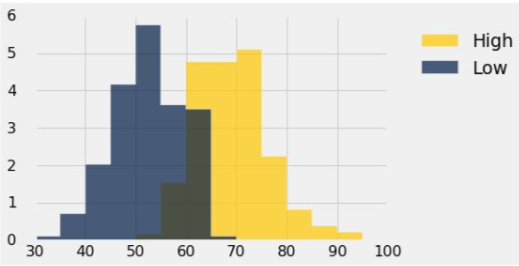
\includegraphics[width = 0.85\textwidth]{hist_high_low.png}
\end{center}
}


%%%SLIDE
\frame{
\begin{center}
\huge \tt  Defining Functions
\end{center}
}



%%%SLIDE
\frame{
{Def Statements}
User-defined functions give names to blocks of code

\begin{center}
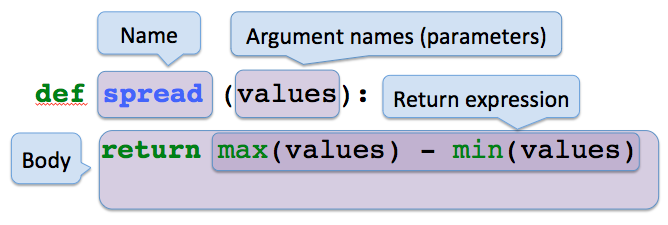
\includegraphics[width=.95\textwidth]{def_statement.png} 
\end{center}
\vfill
\begin{center}
\alert{(DEMO)}
\end{center}
}


%%%SLIDE
\frame{
{Discussion Question}
What does this function do? What kind of input does it take? What output will it give? What's a reasonable name?
\bigskip

\begin{center}
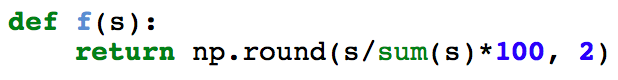
\includegraphics[width=\textwidth]{np_round.png} 
\end{center}
\vfill
\begin{center}
\alert{(DEMO)}
\end{center}
}


%%%SLIDE
\frame{
\begin{center}
\huge \tt  Apply
\end{center}
}



%%%SLIDE
\frame{
{Apply}
The {\tt  \color{Blue} apply} method creates an array by calling a function on every element in input column(s)
\begin{customlist}{2em}{0em}
\item First argument: \quad \quad Function to apply
\item Other arguments: \quad The input column(s)
\end{customlist}

{\color{Blue} \tt
\begin{center}
table\_name.apply(function\_name, `column\_label')
\end{center}}
\vfill
\begin{center}
\alert{(DEMO)}
\end{center}
}

%%%SLIDE
\frame{
\begin{center}
\huge \tt  Example:  Prediction
\end{center}
}



%%%SLIDE
\frame{
{Sir Francis Galton}

\begin{minipage}{0.6\textwidth}
\begin{itemize}
\item 1822 - 1911 (knighted in 1909)
\item A pioneer in making predictions
\item  Particular (and troublesome)
interest in heredity
\item Charles Darwin's half-cousin
\end{itemize}
\begin{center}
\alert{(DEMO)}
\end{center}
\end{minipage}
%
\begin{minipage}{0.38\textwidth} \centering
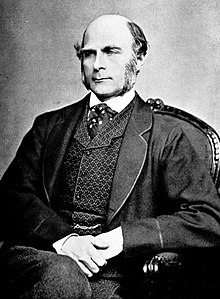
\includegraphics[width = \textwidth]{francis_galton.png}
\end{minipage}

}





%\frame{ 
%{References} \footnotesize
%\bibliographystyle{$HOME/YData/bibliography/asa}
%\bibliography{$HOME/YData/bibliography/ydata_bibliography}
%}




\end{document}
